\chapter{Introduzione ai Sistemi Elettrici per l'Energia}
La maggior parte dell'energia richiesta dalle utenze industriali e civili viene prodotta, trasmessa e utilizzata sotto forma elettrica. 

Il vincolo tecnologico primario dell'energia elettrica risiede nella difficoltà e costi di immagazzinamento. Di conseguenza, il sistema deve garantire istante per istante il bilancio tra la potenza generata e la potenza richiesta dalle utenze: l'energia deve essere generata nello stesso momento in cui viene assorbita.

\section{Diagramma di Carico e Gestione della Produzione}
L'insieme delle utenze connesse alla rete nazionale può essere schematizzato come un unico carico equivalente. La richiesta complessiva di potenza in funzione del tempo viene rappresentata mediante il diagramma di carico. 
\begin{figure}[H]
	\centering
	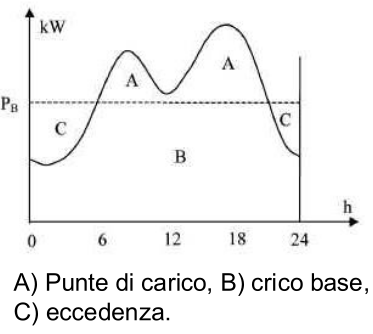
\includegraphics[width=0.4\linewidth]{immagini/introduzione1}
\end{figure}

L'andamento del diagramma di carico presenta una marcata ciclicità giornaliera e stagionale:
\begin{itemize}
    \item Profilo dei giorni feriali $\rightarrow$ caratterizzato da due massimi relativi (punte di carico mattutina e serale), una rampa di incremento rapido della potenza nelle prime ore della giornata (in corrispondenza dell'avvio delle attività produttive e commerciali) e un minimo notturno (valle di carico).
    \item Profilo dei giorni festivi e prefestivi $\rightarrow$ andamento qualitativamente analogo ma con livelli di potenza complessivamente ridotti per la contrazione delle attività lavorative.
\end{itemize}
\newpage
Nel diagramma di carico si distinguono tre aree caratteristiche:
\begin{itemize}
    \item \textbf{Punte di carico (A)} $\rightarrow$ aliquote di potenza variabili eccedenti il livello di carico continuativo, concentrate nelle ore di massimo assorbimento.
    \item \textbf{Carico base (B)} $\rightarrow$ potenza assorbita in modo pressoché costante durante l'intero arco delle 24 ore, indicata con $P_B$.
    \item \textbf{Eccedenza di potenza (C)} $\rightarrow$ margine di potenza disponibile non richiesta dalla rete durante le ore di valle notturna.
\end{itemize}

Per limitare l'escursione tra punte e valli di carico sono state introdotte strutture tariffarie differenziate in fasce orarie. Applicando costi energetici inferiori nelle ore notturne e nei giorni festivi si incentiva lo spostamento dei consumi verso le valli, favorendo l'appiattimento della curva di carico a beneficio della regolarità di esercizio degli impianti.

L'adeguamento continuo della produzione alla curva di carico viene attuato impiegando diverse tipologie di centrali in funzione della loro rapidità di risposta dinamica:
\begin{itemize}
    \item \textbf{Centrali per il servizio di base} $\rightarrow$ tipicamente impianti termoelettrici, caratterizzati da tempi di avviamento lunghi (dell'ordine delle ore) e idonei all'erogazione continuativa della potenza di base $P_B$.
    \item \textbf{Centrali per il servizio di punta} $\rightarrow$ tipicamente impianti idroelettrici a serbatoio o bacino, caratterizzati da tempi di avviamento molto brevi (dell'ordine dei minuti) e capaci di inseguire prontamente le variazioni repentine del carico e coprire le punte.
    \item \textbf{Centrali idroelettriche di produzione e pompaggio} $\rightarrow$ operano su un ciclo a due fasi per valorizzare l'eccedenza notturna $P < P_B$:
    \begin{enumerate}
        \item Fase di pompaggio: nelle ore notturne di minima richiesta, la potenza in eccedenza $C$ generata dagli impianti di base viene impiegata per pompare acqua dal bacino inferiore al bacino superiore, immagazzinando energia sotto forma potenziale idraulica.
        \item Fase di produzione: nelle ore diurne di punta, l'acqua accumulata nel bacino superiore viene rilasciata verso il bacino inferiore attraverso turbine idrauliche calettate agli alternatori, erogando rapidamente potenza attiva alla rete.
        \begin{figure}[H]
        	\centering
        	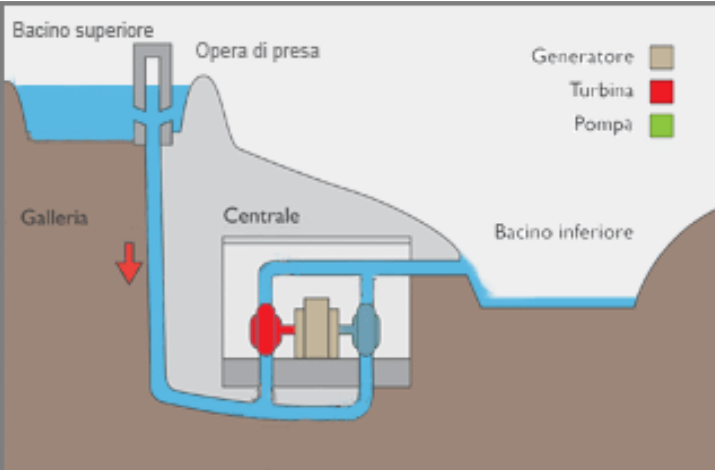
\includegraphics[width=0.4\linewidth]{immagini/introduzione2}
        \end{figure}
        
    \end{enumerate}
\end{itemize}

\newpage
L'esercizio economico e la sicurezza della rete richiedono previsioni accurate del diagramma di carico su base oraria. Il mancato allineamento tra la \textbf{curva di previsione} e il \textbf{diagramma consuntivo} reale obbliga il gestore a reperire energia integrativa in tempo reale a costi sensibilmente più onerosi rispetto al mercato ordinario. Tale programmazione diviene progressivamente più complessa per effetto della penetrazione delle fonti rinnovabili caratterizzate da generazione aleatoria.
\begin{figure}[H]
	\centering
	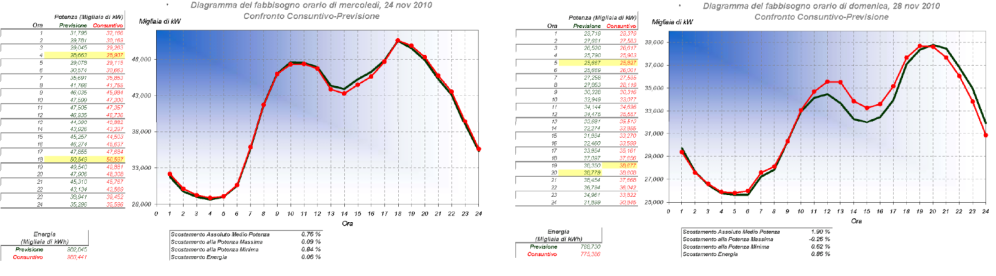
\includegraphics[width=1\linewidth]{immagini/introduzione3}
\end{figure}


\section{Evoluzione del Sistema Elettrico Nazionale}
Il sistema elettrico nazionale è storicamente strutturato secondo un assetto gerarchico composto da quattro subsistemi: produzione, trasmissione, distribuzione e utilizzazione. L'intero complesso è sottoposto al controllo in tempo reale da parte di centri di supervisione e telecontrollo, dove convergono le misure di rete e da cui partono i comandi per il dispacciamento ottimale.

Il settore dell'energia elettrica ha attraversato e continua a registrare una transizione profonda rispetto all'assetto originario:
\begin{itemize}
    \item \textbf{Assetto societario e regolatorio} $\rightarrow$ passaggio da una struttura monopolistica verticalmente integrata (storicamente gestita dall'ente di stato ENEL) a un assetto deregolamentato e disaggregato (\textit{unbundled}) con separazione societaria tra attività di produzione, trasmissione e distribuzione.
    \item \textbf{Topologia della generazione} $\rightarrow$ transizione da una configurazione centralizzata (grandi poli termoelettrici e idroelettrici con flussi di potenza rigidamente unidirezionali verso i carichi) a una decentralizzata, caratterizzata da una marcata diffusione capillare di impianti di generazione distribuita.
    \item \textbf{Dinamica e regolazione di rete} $\rightarrow$ nei sistemi tradizionali la dinamica di rete era governata dalla cospicua inerzia fisica dei grandi generatori sincroni rotanti, in grado di limitare intrinsecamente le variazioni transitorie di frequenza. Nei sistemi moderni la quota predominante della nuova potenza installata è interfacciata tramite convertitori statici (inverter), privi di inerzia meccanica propria, modificando radicalmente le risposte dinamiche del sistema.
    \item \textbf{Criterio di dispacciamento} $\rightarrow$ passaggio da un ordine di merito (\textit{merit order}) rigidamente determinato dai costi marginali dei combustibili fossili a un mercato fortemente influenzato da impianti rinnovabili (eolico e fotovoltaico) operanti con costo marginale della fonte nullo.
    \item \textbf{Comportamento della domanda} $\rightarrow$ transizione da carichi passivi a una domanda attiva (\textit{active demand}), in cui le utenze partecipano alla flessibilità di rete e alla fornitura di servizi ancillari.
    \item \textbf{Strumenti di controllo} $\rightarrow$ evoluzione dai tradizionali sistemi di telecontrollo verso una gestione di rete intelligente supportata da tecnologie digitali, ICT, gestione di grandi moli di dati (\textit{big data}) e algoritmi avanzati.
\end{itemize}

\newpage
\section{Confronto Tecnologico: Corrente Alternata Trifase, Monofase e Corrente Continua}
Il trasferimento di potenza dai siti di produzione ai centri di utilizzazione si effettua in prevalenza mediante sistemi trifase in corrente alternata. 

L'impiego della corrente alternata rispetto alla corrente continua è motivato da precisi vantaggi tecnico-economici:
\begin{itemize}
    \item \textbf{Impiego del trasformatore} $\rightarrow$ macchina elettrica statica fondata sulla legge dell'induzione elettromagnetica (variazione nel tempo del flusso magnetico concatenato). Permette di adattare con estrema semplicità ed elevato rendimento i livelli di tensione più convenienti per ciascuna fase (generazione, trasmissione, distribuzione e utilizzazione).
    \item \textbf{Interruzione delle correnti} $\rightarrow$ nei sistemi in corrente alternata il valore istantaneo della corrente attraversa naturalmente lo zero a ogni semiperiodo ($100$ volte al secondo a $50\text{ Hz}$). Ciò favorisce l'estinzione tempestiva dell'arco elettrico all'interno degli apparecchi di manovra e interruzione, consentendo di interrompere le correnti di cortocircuito prima che provochino danneggiamenti meccanici e termici distruttivi ai dispositivi.
    \item \textbf{Generatore sincrono} $\rightarrow$ macchina ad alta affidabilità rispetto alle macchine a corrente continua (dinamo), grazie all'assenza del collettore meccanico a lamelle, risultando perfettamente idonea all'accoppiamento con turbine a vapore e a gas operanti ad alte velocità di rotazione.
    \item \textbf{Economicità della trasmissione sotto i $1000\text{ km}$} $\rightarrow$ pur presentando maggiori perdite a parità di tensione concatenata e richiedendo una maggiore sezione conduttrice complessiva rispetto a una tratta in continua, il collegamento in alternata non richiede le onerose stazioni terminali di conversione AC/DC e DC/AC.
\end{itemize}

L'efficienza del trasporto di energia su grandi distanze richiede l'innalzamento della tensione. Considerando una linea trifase simmetrica ed equilibrata che trasporta una potenza attiva $P$ con fattore di potenza $\cos\varphi$, la relazione tra le grandezze è data da:
\[P = 3 E I \cos\varphi = \sqrt{3} V I \cos\varphi\]
dove $E$ indica il modulo della tensione stellata (fase-neutro), $V = \sqrt{3} E$ il modulo della tensione concatenata (fase-fase) e $I$ la corrente di linea.

La corrente di linea risulta pari a:
\[I = \frac{P}{\sqrt{3} V \cos\varphi}\]

Le perdite di potenza per effetto Joule dissipative lungo la linea trifase avente resistenza per fase pari a $R$ sono espresse da:
\[\Delta P = 3 R I^2 = 3 R \left( \frac{P}{\sqrt{3} V \cos\varphi} \right)^2 = \frac{R P^2}{V^2 \cos^2\varphi}\]

Se si incrementa la tensione concatenata di un fattore $k$ mediante l'inserimento di trasformatori:
\[V' = k V \implies I' = \frac{I}{k} \implies \Delta P' = \frac{\Delta P}{k^2}\]
A parità di potenza attiva trasmessa, un incremento della tensione concatenata di un fattore pari a $10$ determina la diminuzione della corrente di linea di un fattore $10$ e la contestuale riduzione delle perdite dissipative per effetto Joule di un fattore pari a $100$.

\newpage
L'adozione della configurazione trifase rispetto a quella monofase è dettata da tre vantaggi fondamentali:
\begin{itemize}
    \item \textbf{Motore asincrono trifase} $\rightarrow$ capacità intrinseca di generare un campo magnetico rotante nello statore, garantendo maggiore semplicità costruttiva, sicurezza di funzionamento, rendimento ed economicità rispetto al motore monofase.
    \item \textbf{Generatore sincrono trifase} $\rightarrow$ notevoli vantaggi dimensionali, costruttivi e di bilanciamento delle coppie resistenti rispetto al generatore monofase.
    \item \textbf{Minori cadute di tensione e costi di linea} $\rightarrow$ a parità di potenza attiva trasmessa e di perdite dissipative, il sistema trifase richiede una quantità di materiale conduttore inferiore rispetto a sistemi monofase equivalenti.
\end{itemize}

I sistemi monofase e a corrente continua trovano impiego in contesti specifici:
\begin{itemize}
    \item \textbf{Corrente alternata monofase} $\rightarrow$ utilizzata nella trazione elettrica ferroviaria e nella fase finale di distribuzione in bassa tensione per l'alimentazione delle utenze domestiche ($230\text{ V}$ tra fase e neutro).
    \item \textbf{Corrente continua (HVDC)} $\rightarrow$ utilizzata nelle trasmissioni terrestri su distanze superiori a circa $1000\text{ km}$ (dove i minori costi dei conduttori e le inferiori perdite compensano il costo delle stazioni di conversione) e nei collegamenti sottomarini in cavo, dove è possibile utilizzare l'acqua di mare come conduttore di ritorno con rilevanti economie impiantistiche.
\end{itemize}

\section{Classificazione dei livelli di tensione}
Nei sistemi elettrici di potenza la tensione nominale $V_n$ assume valori differenziati in base alla funzione di rete. Si distinguono due classificazioni fondamentali: quella di uso corrente (tecnica) e quella normativa (norme CEI).

La classificazione di uso corrente ripartisce i livelli di tensione in quattro fasce:
\begin{itemize}
    \item \textbf{Bassa Tensione (bt)} $\rightarrow$ $V_n \le 1000\text{ V}$ ($1\text{ kV}$).
    \item \textbf{Media Tensione (MT)} $\rightarrow$ $1000\text{ V} < V_n \le 30\,000\text{ V}$ ($1\text{ kV} < V_n \le 30\text{ kV}$).
    \item \textbf{Alta Tensione (AT)} $\rightarrow$ $30\,000\text{ V} < V_n \le 150\,000\text{ V}$ ($30\text{ kV} < V_n \le 150\text{ kV}$).
    \item \textbf{Altissima Tensione (AAT)} $\rightarrow$ $V_n \ge 150\,000\text{ V}$ ($150\text{ kV}$).
\end{itemize}

La classificazione normativa definita dalle norme CEI suddivide i sistemi in categorie in funzione della tensione nominale tra le fasi o verso terra, distinguendo tra corrente alternata e corrente continua:
\begin{itemize}
    \item \textbf{Categoria 0} $\rightarrow$ per tensioni alternate $V_n \le 50\text{ V}$, per tensioni continue $V_n \le 120\text{ V}$.
    \item \textbf{Categoria 1} $\rightarrow$ per tensioni alternate $50\text{ V} < V_n \le 1000\text{ V}$, per tensioni continue $120\text{ V} < V_n \le 1500\text{ V}$.
    \item \textbf{Categoria 2} $\rightarrow$ per tensioni alternate $1000\text{ V} < V_n \le 30\,000\text{ V}$, per tensioni continue $1500\text{ V} < V_n \le 30\,000\text{ V}$.
    \item \textbf{Categoria 3} $\rightarrow$ per tensioni alternate $V_n > 30\,000\text{ V}$, per tensioni continue $V_n > 30\,000\text{ V}$.
\end{itemize}

\newpage
\section{Architettura e subsistemi del sistema elettrico per l'energia}
La struttura gerarchica del sistema elettrico per l'energia si articola nei seguenti subsistemi interconnessi:
\begin{figure}[H]
	\centering
	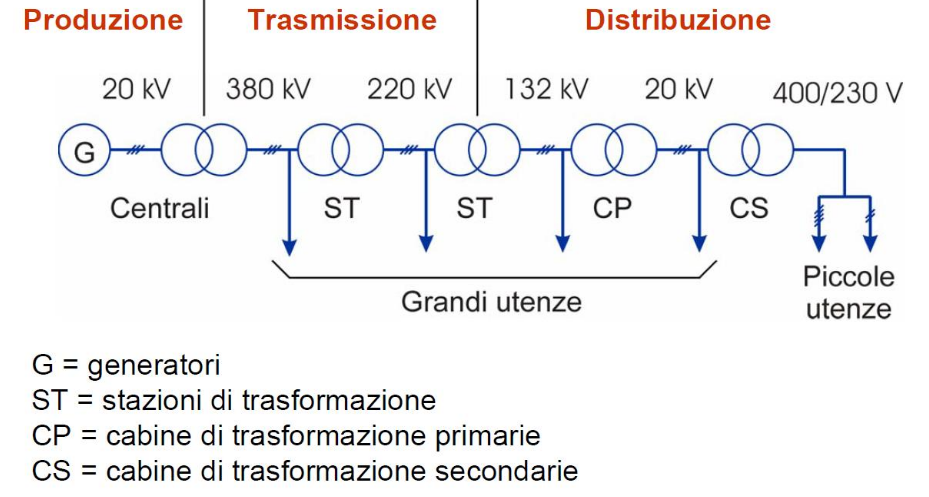
\includegraphics[width=0.8\linewidth]{immagini/introduzione4}
\end{figure}

\subsection{Subsistema di produzione}
Nel subsistema di produzione l'energia elettrica viene generata convertendo fonti di energia primaria: energia idraulica (impianti idroelettrici), energia termica da combustibili fossili (impianti termoelettrici a carbone, gas naturale, derivati del petrolio), combustibili nucleari (assenti nel parco produttivo nazionale), vapori naturali del sottosuolo (impianti geotermoelettrici), energia solare (impianti fotovoltaici) ed energia eolica.

Le caratteristiche costruttive e di connessione del subsistema di produzione sono le seguenti:
\begin{itemize}
    \item \textbf{Alternatori trifase} $\rightarrow$ la generazione avviene mediante generatori sincroni con frequenza nominale di $50\text{ Hz}$ e tensioni nominali dell'ordine di decine di kilovolt (tipicamente nell'intervallo $15 \div 20\text{ kV}$).
    \item \textbf{Stazioni di trasformazione annesse alle centrali} $\rightarrow$ i generatori sono connessi alle linee di trasmissione mediante trasformatori elevatori a rapporto fisso. L'impiego del rapporto fisso (senza commutatori sotto carico) è giustificato dal fatto che la regolazione della tensione ai morsetti viene effettuata direttamente agendo sulla corrente di eccitazione dei generatori sincroni.
    \item \textbf{Criteri di allacciamento alla rete in base alla potenza nominale}:
    \begin{itemize}
        \item Centrali con potenza superiore a $250\text{ MVA}$ $\rightarrow$ connesse tassativamente alle linee ad altissima tensione a $380\text{ kV}$ o $220\text{ kV}$.
        \item Centrali con potenza inferiore a $250\text{ MVA}$ $\rightarrow$ connesse alle linee a $380\text{ kV}$, $220\text{ kV}$ o direttamente alle linee di subtrasmissione a $132\text{ kV}$.
        \item Centrali di taglia ridotta con potenza inferiore a $10\text{ MVA}$ $\rightarrow$ possono essere collegate direttamente alle reti di distribuzione in media tensione (MT).
    \end{itemize}
\end{itemize}

\newpage
\subsection{Subsistema di trasmissione}
Il subsistema di trasmissione ha il compito di trasportare all'ingrosso grandi blocchi di potenza dalle centrali di produzione ai centri di trasformazione e consumo distribuiti sul territorio nazionale.

Le caratteristiche della rete di trasmissione sono:
\begin{itemize}
    \item \textbf{Configurazione magliata} $\rightarrow$ la rete presenta una struttura a maglie chiuse i cui rami sono linee elettriche aeree trifase senza conduttore di neutro. La configurazione magliata garantisce elevata affidabilità ed elevata continuità di servizio rispetto a una rete radiale: in caso di disconnessione o guasto su una linea, l'alimentazione dei nodi permane attraverso i rami alternativi della maglia.
    \begin{figure}[H]
    	\centering
    	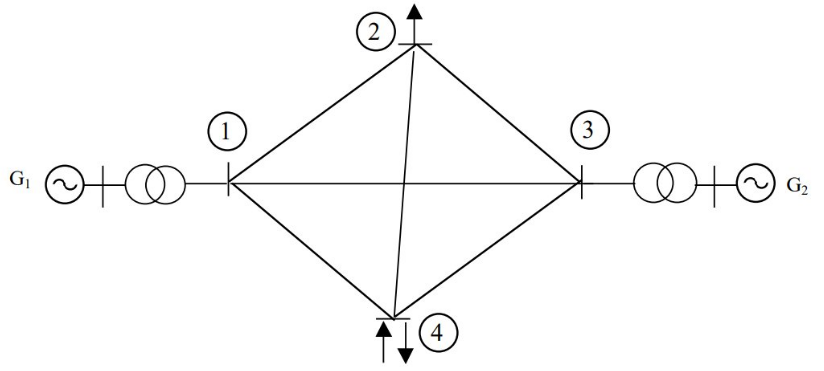
\includegraphics[width=0.5\linewidth]{immagini/introduzione5}
    \end{figure}
    \item \textbf{Livelli di tensione} $\rightarrow$ la rete è esercita alla tensione nominale di $380\text{ kV}$ (dorsale ad altissima tensione di estensione nazionale) e a $220\text{ kV}$ (rete di subtrasmissione a estensione regionale). L'interconnessione tra le sezioni a $380\text{ kV}$ e a $220\text{ kV}$ è realizzata tramite autotrasformatori disposti nelle stazioni di trasformazione.
    \item \textbf{Stazioni primarie} $\rightarrow$ nodi di interfaccia tra la trasmissione e la distribuzione. La trasformazione avviene mediante autotrasformatori abbassatori dotati di regolazione del rapporto di trasformazione variabile sotto carico (LTC), indispensabili per svincolare e isolare le variazioni di tensione della rete a $380\text{ kV}$ dai livelli di tensione delle reti di distribuzione a valle.
    \item \textbf{Collegamenti in corrente continua (HVDC)} $\rightarrow$ la rete di trasmissione italiana include collegamenti sottomarini a corrente continua:
    \begin{itemize}
        \item Cavo sottomarino a $\pm 500\text{ kV}$ in corrente continua tra la penisola italiana e la Sardegna (collegamento SAPEI).
        \item Cavo sottomarino a $200\text{ kV}$ in corrente continua tra Toscana, Corsica e Sardegna (collegamento SACOI).
        \item Cavo sottomarino in corrente continua di interconnessione tra l'Italia e la Grecia.
    \end{itemize}
    \item \textbf{Interconnessioni internazionali} $\rightarrow$ la rete italiana è interconnessa mediante linee sincrone ad alta tensione con le reti delle nazioni confinanti (Francia, Svizzera, Austria e Slovenia). A livello europeo le reti di trasmissione sono storicamente confluite in blocchi operativi sincroni: blocco UCPTE (Europa occidentale), NORDEL (paesi scandinavi: Svezia, Norvegia, Finlandia) ed ex-COMECON (Europa orientale), tra loro interconnessi con collegamenti sottomarini e stazioni di conversione terrestri. In Italia la gestione e il dispacciamento della Rete di Trasmissione Nazionale (RTN) sono affidati al Gestore di Rete (Terna).
\end{itemize}

Nello schema di principio a 4 nodi, la rete magliata collega:
\begin{itemize}
    \item Nodi 1 e 3 $\rightarrow$ nodi di immissione di potenza dalle centrali di generazione dopo trasformazione a rapporto fisso.
    \item Nodo 2 $\rightarrow$ nodo di trasferimento di potenza al subsistema di distribuzione attraverso la stazione primaria.
    \item Nodo 4 $\rightarrow$ nodo di interconnessione con una rete estera per lo scambio bidirezionale di energia.
\end{itemize}

\subsection{Subsistema di distribuzione}
Il subsistema di distribuzione ha il compito di prelevare la potenza dalle stazioni primarie della trasmissione e capillarizzarla fino ai singoli utilizzatori finali. Si articola in tre livelli a cascata:
\begin{itemize}
    \item \textbf{Reti di distribuzione primaria} $\rightarrow$ esercite in alta tensione alla tensione nominale di $150\text{ kV}$ o $132\text{ kV}$, alimentate dalle stazioni primarie connesse alla rete a $380\text{ kV}$.
    \item \textbf{Reti di distribuzione a media tensione (MT)} $\rightarrow$ esercite alla tensione nominale di $20\text{ kV}$, originano dalle stazioni di trasformazione AT/MT e alimentano le cabine secondarie e le medie utenze.
    \item \textbf{Reti di distribuzione a bassa tensione (BT)} $\rightarrow$ esercite alla tensione nominale trifase concatenata di $400\text{ V}$ (tensione stellata di $230\text{ V}$, storicamente $380/220\text{ V}$), alimentate dalle cabine di trasformazione MT/BT. La linea a bassa tensione è distribuita mediante $4$ conduttori: tre conduttori di fase e il conduttore di neutro.
\end{itemize}

Le configurazioni topologiche della distribuzione dipendono dalla densità di carico e dal livello richiesto di continuità del servizio:
\begin{itemize}
    \item Configurazione magliata $\rightarrow$ adottata in aree urbane ad elevata densità di carico dove sono richieste minime interruzioni di servizio.
    \item Configurazione radiale (ad albero) $\rightarrow$ adottata per l'estensione su ampie aree e zone rurali per contenere i costi di impianto; il flusso di potenza è unidirezionale, con origine dalla stazione di alimentazione e propagazione verso i terminali.
\end{itemize}
\begin{figure}[H]
	\centering
	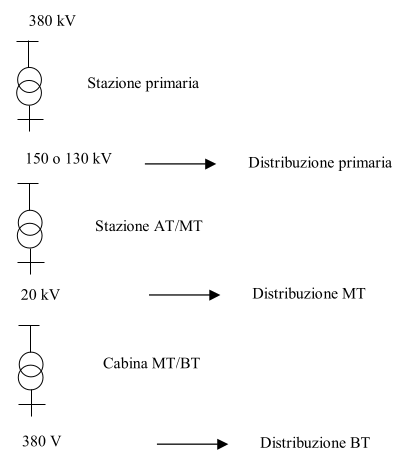
\includegraphics[width=0.5\linewidth]{immagini/introduzione6}
\end{figure}
\newpage
\subsection{Subsistema di utilizzazione}
Il subsistema di utilizzazione è costituito dall'insieme dei carichi e delle utenze allacciate alla rete. Il punto di fornitura e il relativo livello di tensione dipendono dalla potenza assorbita:
\begin{itemize}
    \item \textbf{Grandi utenze industriali e trazione ferroviaria} $\rightarrow$ connesse direttamente in alta o altissima tensione alle stazioni primarie ($380\text{ kV}$, $220\text{ kV}$) o alle stazioni della distribuzione primaria ($150\text{ kV}$ o $132\text{ kV}$).
    \item \textbf{Medie utenze industriali e commerciali} $\rightarrow$ connesse alla rete di media tensione ($20\text{ kV}$) a partire dalle stazioni AT/MT.
    \item \textbf{Piccole utenze civili, commerciali e domestiche} $\rightarrow$ connesse alla rete di bassa tensione ($400\text{ V}$ trifase o $230\text{ V}$ monofase) a partire dalle cabine secondarie MT/BT.
\end{itemize}

\section{Componenti del sistema elettrico per l'energia}
L'architettura del sistema elettrico per l'energia si compone di elementi circuitali fondamentali e di dispositivi ausiliari di manovra e controllo:
\begin{itemize}
    \item \textbf{Generatori sincroni} $\rightarrow$ conversione dell'energia meccanica fornita dalle turbine in energia elettrica trifase.
    \item \textbf{Trasformatori e autotrasformatori} $\rightarrow$ accoppiamento magnetico tra sezioni di rete a diverso livello di tensione per l'adattamento delle grandezze e l'abbattimento delle correnti.
    \item \textbf{Linee elettriche} $\rightarrow$ linee aeree su sostegni o cavi interrati/sottomarini per il convogliamento della corrente.
    \item \textbf{Carichi} $\rightarrow$ utilizzatori civili e industriali che assorbono potenza attiva e reattiva convertendola in lavoro o calore.
\end{itemize}

A questi si affiancano i componenti preposti all'esercizio, alla protezione e al controllo:
\begin{itemize}
    \item \textbf{Apparecchi di manovra} $\rightarrow$ interruttori capaci di aprire e chiudere circuiti sotto carico e in presenza di cortocircuito; sezionatori preposti all'isolamento visibile di tratte circuitali prive di corrente.
    \item \textbf{Apparecchi di misura} $\rightarrow$ riduttori di corrente (TA) e riduttori di tensione (TV) per il rilievo delle grandezze di rete e l'isolamento della strumentazione.
    \item \textbf{Apparecchi di regolazione} $\rightarrow$ regolatori di velocità delle turbine per il controllo della frequenza e regolatori automatici di tensione (AVR) agenti sull'eccitazione degli alternatori.
    \item \textbf{Relè e sistemi di protezione} $\rightarrow$ rivelazione selettiva delle condizioni anormali di guasto e trasmissione del comando di scatto agli organi di manovra.
    \item \textbf{Sistemi elettronici di potenza} $\rightarrow$ convertitori statici, inverter e raddrizzatori per il controllo del flusso di potenza e l'interfacciamento delle sorgenti non sincrone.
\end{itemize}

\section{Condizioni di funzionamento del sistema elettrico}
Il funzionamento del sistema elettrico per l'energia si suddivide in due regimi operativi fondamentali: funzionamento normale e funzionamento anormale.

\subsection{Condizioni di funzionamento normali}
Nel funzionamento normale tutte le grandezze elettriche del sistema a regime stazionario (tensioni, correnti, frequenza) sono racchiuse all'interno di intervalli ammessi per il corretto esercizio delle macchine e degli impianti. In particolare, la frequenza è mantenuta in prossimità del valore nominale di $50\text{ Hz}$ e le tensioni rimangono comprese entro una fascia di tolleranza ristretta pari a $\pm 5\% \div \pm 10\%$ attorno al valore nominale.

Nel funzionamento normale si pongono i seguenti problemi tecnici fondamentali come regolazione della frequenza, regolazione della tensione e ripartizione attive e reattive tra i vari impianti di produzione.

\section{Condizioni di funzionamento anormali}
Le condizioni di funzionamento anormale sono determinate da scostamenti marcati delle correnti o delle tensioni rispetto ai valori nominali. Si distinguono sovracorrenti (correnti superiori alla portata nominale dei conduttori) e sovratensioni.

Esiste anche una condizione di funzionamento anormale in un circuito elettricamente “sano”, in presenza di disturbi della tensione.

\subsection{Sovracorrenti}
La portata nominale rappresenta il massimo valore di corrente che un componente o conduttore può sopportare in regime continuativo senza che la temperatura superi i limiti ammissibili per i materiali isolanti. In base allo stato del circuito si distinguono due tipologie di sovracorrente:
\begin{itemize}
    \item \textbf{Corrente di sovraccarico} $\rightarrow$ si manifesta in un circuito elettricamente sano; deriva da un assorbimento di potenza da parte dei carichi eccedente la capacità nominale della tratta.
    \item \textbf{Corrente di cortocircuito} $\rightarrow$ si manifesta in un circuito elettricamente guasto; deriva dal cedimento dell'isolamento e dall'instaurarsi di un percorso di guasto.
\end{itemize}

\subsection{Cortocircuito}
Il cortocircuito è la condizione anormale provocata da un collegamento a bassa impedenza che viene ad instaurarsi accidentalmente fra i conduttori di fase, tra conduttori e terra, o fra parti a differente potenziale di macchine e apparecchiature.

Le caratteristiche del cortocircuito sono:
\begin{itemize}
    \item \textbf{Impedenza di guasto}:
    \begin{itemize}
        \item Cortocircuito netto $\rightarrow$ impedenza nel punto di contatto rigorosamente nulla o trascurabile.
        \item Cortocircuito tramite impedenza $\rightarrow$ contatto stabilito attraverso un'impedenza non trascurabile (ad esempio per interposizione di un arco elettrico o resistenza di contatto verso terra).
    \end{itemize}
    \item \textbf{Classificazione in base alle fasi e al coinvolgimento della terra}:
    \begin{itemize}
        \item Cortocircuito trifase $\rightarrow$ guasto che interessa contemporaneamente tutte e tre le fasi del circuito. È un \textbf{guasto simmetrico} in quanto non altera la terna simmetrica delle impedenze di linea.
        \item Cortocircuito bifase $\rightarrow$ guasto tra due fasi del circuito, che può avvenire isolato da terra o franco a terra. È un \textbf{guasto dissimmetrico}.
        \item Cortocircuito monofase $\rightarrow$ guasto che si stabilisce tra un singolo conduttore di fase e la terra. È un guasto dissimmetrico ed è la tipologia statisticamente più frequente negli impianti ad alta tensione.
    \end{itemize}
    \newpage
    \item \textbf{Sollecitazioni associate alle correnti di cortocircuito}:
    \begin{itemize}
        \item Sollecitazione termica $\rightarrow$ riscaldamento dei conduttori con pericolo di degrado termico immediato degli isolamenti.
        \item Sollecitazione elettrodinamica $\rightarrow$ insorgenza di forze meccaniche tra conduttori, con rischio di deformazione irreversibile o rottura meccanica di sbarre, isolatori e sostegni.
    \end{itemize}
    \item \textbf{Problematiche tecniche connesse}:
    \begin{itemize}
        \item Scelta degli interruttori di manovra e protezione.
        \item Dimensionamento degli impianti di terra.
        \item Verifica della stabilità del moto rotatorio dei generatori sincroni.
    \end{itemize}
\end{itemize}

\subsection{Sovratensioni}
Si definisce sovratensione qualsiasi incremento del valore istantaneo o efficace della tensione tra due fasi o tra una fase e la terra che superi la soglia massima prevista per il funzionamento normale (eccedente l'intervallo di tolleranza $\pm 5\% \div \pm 10\%$ attorno alla tensione nominale $V_n$).

In base all'origine fisica si distinguono:
\begin{itemize}
    \item \textbf{Sovratensioni di origine interna} $\rightarrow$ derivano da cause connesse all'esercizio del sistema (manovre su circuiti reattivi, disconnessioni di carico, anomalie, guasti); la loro ampiezza è direttamente proporzionale alla tensione nominale $V_n$ dell'impianto.
    \item \textbf{Sovratensioni di origine esterna} $\rightarrow$ derivano da fenomeni atmosferici (scariche fulminee dirette o accoppiamenti induttivi ed elettrostatici); l'ampiezza delle tensioni generate è totalmente indipendente dalla tensione nominale $V_n$ dell'impianto.
\end{itemize}

In relazione alla forma d'onda e alla durata temporale, le sovratensioni vengono classificate in:
\begin{itemize}
    \item \textbf{Sovratensioni atmosferiche} $\rightarrow$ causate da fulminazione diretta dei conduttori aerei nudi o da induzione elettromagnetica dovuta a scariche nube-terra in prossimità della linea. Sono caratterizzate da onde impulsive unidirezionali di breve durata (fronte di salita dell'ordine dei microsecondi e durata complessiva al più di qualche centinaio di $\mu\text{s}$). Provocano tensioni di picco che possono raggiungere $1000\text{ kV}$ con correnti di scarica fino a $200\text{ kA}$.
    \item \textbf{Sovratensioni di manovra} $\rightarrow$ originate dall'apertura o chiusura di organi di interruzione (manovra di banchi di condensatori, apertura di linee a vuoto con interruzione di correnti capacitive, distacco di carichi altamente induttivi o richiusura rapida di linee). Sono caratterizzate da onde oscillanti fortemente smorzate, assimilabili a impulsi unidirezionali di durata compresa tra millisecondi e decimi di secondo. Si distinguono in normali o anormali a seconda che il valore di picco risulti inferiore o superiore al doppio della tensione di riferimento di fase $v_{pr}$:
    \[v_{pr} = \sqrt{2} \, \frac{U_x}{\sqrt{3}}\]
    essendo $U_x$ il valore efficace della tensione concatenata nominale dell'impianto.
    \item \textbf{Sovratensioni sostenute} $\rightarrow$ originate da manovre di eliminazione dei guasti, risonanze su frequenze armoniche o fenomeni di ferrorisonanza (interazione non lineare tra induttanze saturabili di trasformatori e capacità di linea). Sono costituite da onde oscillanti debolmente smorzate a frequenza industriale ($50\text{ Hz}$) o armonica, altamente pericolose per l'elevato contenuto energetico prolungato nel tempo.
\end{itemize}

\newpage
Le sovratensioni causano sollecitazioni anormali sugli isolamenti dei diversi componenti del sistema e
possono provocare corto circuiti.

Per preservare l'integrità degli isolamenti si adottano criteri di coordinamento dell'isolamento e l'installazione di scaricatori di sovratensione (SPD):
\begin{itemize}
    \item \textbf{Scaricatore di sovratensione} $\rightarrow$ componente di protezione collegato tra i conduttori attivi e l'impianto di terra, caratterizzato da una resistenza fortemente non lineare in funzione della tensione applicata:
    \begin{itemize}
        \item In condizioni di tensione normale di esercizio presenta un'impedenza elevatissima, comportandosi circuitalmente come un circuito aperto con assorbimento di corrente trascurabile.
        \item Al manifestarsi di una sovratensione l'impedenza del dispositivo si riduce bruscamente a valori prossimi a zero, comportandosi come un cortocircuito verso terra e drenando la corrente impulsiva, limitando la tensione ai capi dell'apparecchiatura protetta al di sotto della soglia di tenuta dell'isolamento.
    \end{itemize}
\end{itemize}
\begin{figure}[H]
	\centering
	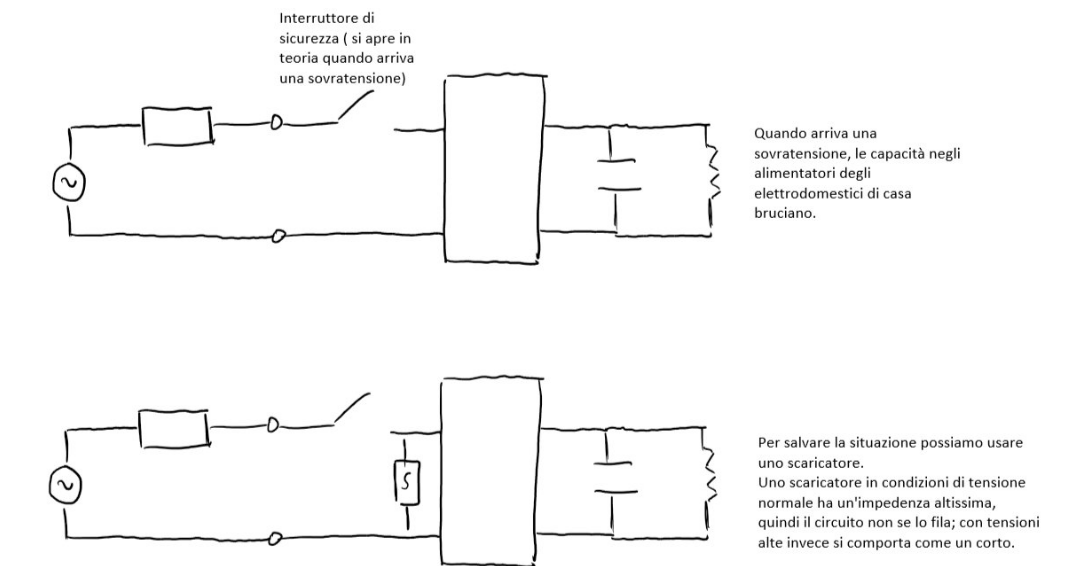
\includegraphics[width=0.85\linewidth]{immagini/introduzione7}
\end{figure}


